
\documentclass[sigconf, review]{acmart}
%%
%% \BibTeX command to typeset BibTeX logo in the docs
\AtBeginDocument{%
  \providecommand\BibTeX{{%
    Bib\TeX}}}

\setcopyright{acmlicensed}
\copyrightyear{2018}
\acmYear{2018}
\acmDOI{XXXXXXX.XXXXXXX}
%% These commands are for a PROCEEDINGS abstract or paper.
\acmConference[Conference acronym 'XX]{Make sure to enter the correct
  conference title from your rights confirmation email}{June 03--05,
  2018}{Woodstock, NY}

\acmISBN{978-1-4503-XXXX-X/2018/06}




\usepackage{graphicx}
\usepackage{amsmath, amssymb}
\usepackage{hyperref}
%\usepackage{cite}
\usepackage{algorithm}
\usepackage{algorithmic}
\usepackage{hyperref}
\usepackage{caption}
\usepackage{subcaption} % For subfigures and side-by-side images
\usepackage{graphicx}
\graphicspath{ {./images/} }
\usepackage{booktabs} % For better table formatting
\usepackage{multirow} % For multirow cells
\usepackage{array} % For custom column alignment
\usepackage{tabularx} % For auto-adjusting table width
\usepackage{booktabs} % For better table formatting
\usepackage{adjustbox} % For scaling the table
\usepackage{geometry} % For better page margins
\usepackage{array}
\usepackage[section]{placeins}
\usepackage[section]{placeins} % for \FloatBarrier
%%
%% end of the preamble, start of the body of the document source.
\begin{document}

%%

\title{SportsOri: A Novel Dataset for Analyzing Public Sentiment on Controversial Sports Events in YouTube Comments}




\author{Yuvraj Singh}
%\authornote{Both authors contributed equally to this research.}
% \email{trovato@corporation.com}
% \orcid{1234-5678-9012}
% \author{G.K.M. Tobin}
% \authornotemark[1]

\affiliation{%
  \institution{IIIT Bhubaneswar}
  \city{Bhubaneswar, Orissa}
  %\state{Ohio}
  \country{India}
}
\email{yuvraj.mist@gmail.com}

\author{Devadripta Jadhav}
\affiliation{%
  \institution{Savitribai Phule Pune University}
  \city{Pune, Maharashtra}
  \country{India}}
\email{devadripta@gmail.com}

\author{Samiksha Boduwar}
\affiliation{%
  \institution{Savitribai Phule Pune University}
  \city{Pune, Maharashtra}
  \country{India}}
\email{samikshaboduwar@gmail.com}




\author{Kripabandhu Ghosh}
\affiliation{%
  \institution{IISER Kolkata}
  \city{Mohanpur, West Bengal}
  \country{India}}
\email{kripaghosh@iiserkol.ac.in}
%%
%% By default, the full list of authors will be used in the page
%% headers. Often, this list is too long, and will overlap
%% other information printed in the page headers. This command allows
%% the author to define a more concise list
%% of authors' names for this purpose.
\renewcommand{\shortauthors}{Singh et al.}

%%
%% The abstract is a short summary of the work to be presented in the
%% article.
\begin{abstract}
  This paper presents an analysis of YouTube comments on famous and controversial Public Sports Events. We explore public sentiment analysis (stance detection) on a total of 6 famous controversial sports incidents by extracting and processing YouTube comments. Stance detection is performed on those events through fine-tuning of models like Llama-3.1-8b and Deepseek reasoning models (Llama-8b distilled) on hand-curated examples like \textit{The Underarm Incident}, \textit{Jonny Bairstow's Run-Out} Incident, \textit{Ashwin's Mankadding} Event, \textit{Luis Suarez Handball} Event etc. Our code is available \footnote{\url{https://github.com/YuvrajSingh-mist/Public-Sports-Controversy}}
The complete event details,  results and evaluation metrics will be discussed in detail in subsequent sections. 
Our models can be found here \footnote{\url{https://huggingface.co/YuvrajSingh9886/Llama3.1-8b-Maradona/}} \footnote{\url{https://huggingface.co/YuvrajSingh9886/Llama3.1-8b-Frank-Lampard/}} \footnote{\url{https://huggingface.co/YuvrajSingh9886/Llama-3.1-8b-Luis-Suarez}}. 
\footnote{\url{https://huggingface.co/YuvrajSingh9886/llama-8b-distill-reasoning-deepseek-frank}}
\footnote{\url{https://huggingface.co/YuvrajSingh9886/llama-8b-distill-reasoning-deepseek-luis}}
\footnote{\url{https://huggingface.co/YuvrajSingh9886/llama-8b-distill-reasoning-deepseek-maradona}} Our entire pipeline can be found here \footnote{\url{https://github.com/YuvrajSingh-mist/Public-Sports-Controversy/tree/master/data/PDFs}}
       
  

\end{abstract}


\begin{CCSXML}
<ccs2012>
   <concept>
       <concept_id>10002951.10003260.10003277</concept_id>
       <concept_desc>Information systems~Web mining</concept_desc>
       <concept_significance>500</concept_significance>
       </concept>
 </ccs2012>
\end{CCSXML}

\ccsdesc[500]{Information systems~Web mining}

\keywords{Stance Detection, YouTube Comments, Social Media Analysis, Sports Controversies}

\maketitle

\section{Introduction}

%Hello~\cite{sportqa}

Sports engages billions of followers worldwide\footnote{\url{https://www.statista.com/chart/14329/global-interest-in-football/}} 
and impacts the economy \cite{sportseconomics20221}. Sports controversies often ignite passionate discussions among fans, analysts, and players. With the rise of social media, platforms like YouTube have become central to these discussions. This study aims to analyze the stances or perform opinion mining namely for, against, and neutral on comments from famous social media platforms like YouTube for famous public sports controversies.
To our knowledge, it is the first-ever study of civic engagement in controversial sports events spans around 40 years. LLMs (Llama and Deepseek reasoning family) were used for initial annotations (stance) of comments and later fine-tuned for comparative performance analysis ($~$30\% boost in accuracy).
This will prove to be useful in benchmarking and evaluation of systems in opinion mining and/or sentiment analysis for consumer systems on social medial to prevent hate speech, discriminatory opinions etc. 


% Sports controversies often ignite passionate discussions among fans, analysts, and players. With the rise of social media, platforms like YouTube have become central to these discussions. This study aims to analyze the stances or perform opinion mining namely for, against, and neutral on comments from famous social media platforms like YouTube, focusing on events such as Jonny Bairstow's Run-Out Incident, Luis Suarez Handball Event etc.
% To our knowledge, the first-ever study of civic engagement in controversial sports events (cricket and football) spans around 40 years. LLMs (Llama3 family) were used for initial annotations (stance) of comments and later fine-tuned for comparative performance analysis ($~$30\% boost in accuracy).%~\cite{Lamport:LaTeX}

Our study stands apart from its counterparts by focusing on public sentiment analysis surrounding controversial sports events, specifically through the lens of YouTube comments. Papers like SportQA \cite{xia-etal-2024-sportqa} aims to evaluate how well large language models (LLMs) understand sports knowledge through a benchmark dataset while Run Like a Girl! \cite{harrison-etal-2023-run} delves into gender bias in sports-related datasets, highlighting under-representation and naming disparities. We shift the focus to how people react to contentious moments in sports. It uses stance detection techniques to analyse public opinion, offering insights into the emotional and polarised responses to events. Moreover, studies like Generating Sports News from Live Commentary \cite{huang-etal-2020-generating} are centred on automating sports news generation from live commentary, emphasising summarisation and natural language generation. In essence, while the other studies explore sports understanding, bias, and news automation, our study uniquely examines the social media-driven public discourse around sports controversies, making it distinct in its focus on human reactions and sentiment. Thus, after a thorough human verification, we are releasing a dataset of 40K+ opinion-labelled comments (Section \ref{sec:dataset}) and discuss the results in Section \ref{sec:res_discuss}. 

% The Frank Lampard "Ghost Goal" during the 2010 World Cup against Germany was a pivotal moment of controversy. The goal was clearly visible on replays as having crossed the line, but referee Jorge Larrionda and assistant Mauricio Espinosa missed it, leading to widespread media coverage and fan outrage 12. This incident was a significant catalyst for the introduction of goal-line technology in football, highlighting the need for technological assistance in critical refereeing decisions35. The decision was seen as a turning point in the match, which England eventually lost 4-12. The controversy overshadowed England's overall performance at the tournament, shifting focus from managerial issues to the refereeing error2.

%\cite{sportqa}
%{\color{red}KRIPA: Cite these https://aclanthology.org/search/?q=sports and explain why our work is different}


\section{Dataset Creation: SportsOpi}\label{sec:dataset}



\subsection{Data Collection}

We first identified famous public sports controversies by randomly picking 100 such events (football and cricket) from Wikipedia \footnote{\url{https://en.wikipedia.org/wiki/Category:Sports_controversies}} 
 and fetching 100 YouTube videos, sorted by "Most relevant" filter, related to each such controversy. Subsequently, the comments were fetched through YouTube Data API \footnote{\url{https://developers.google.com/youtube/v3}}, and sorted in decreasing order of number of comments. Thus, the final controversial events were chosen by considering the total number of samples each event had followed by quality, engagement and balance of polarity. Our methodology focussed on the creation of a curated playlist for each event, ensuring diverse opinions. Since we are looking for public engagement on historic sports controversies, we look for events that have opinions of diverse classes viz. {\bf Favour}, {\bf Against}, {\bf Neutral} and {\bf Irrelevant}. The respective definitions for these labels can be found here.

\subsection{The Events}

Following the data collection pipeline, a total of six events were chosen, namely, \noindent {\bf Frank Lampard Ghost Goal \footnote{\url{https://thesefootballtimes.co/2016/02/28/diego-maradona-and-the-reality-behind-the-hand-of-god/}}}, \noindent {\bf Maradona Hand of God \footnote{\url{https://thesefootballtimes.co/2016/02/28/diego-maradona-and-the-reality-behind-the-hand-of-god/}} }, {\bf Luis Suárez's deliberate handball \footnote{\url{https://www.skysports.com/football/news/12040/12759389/uruguays-luis-suarez-says-he-will-not-apologise-to-ghana-for-his-handball-that-knocked-them-out-of-2010-world-cup}} }, {\bf The Jonny Bairstow Ashes Runout \footnote{\url{https://www.espncricinfo.com/story/jonny-bairstow-reignites-ashes-stumping-row-1405100}}}, {\bf Ravichandran Ashwin's Mankading \footnote{\url{https://www.espncricinfo.com/story/jonny-bairstow-reignites-ashes-stumping-row-1405100}}}, {\bf The Underarm \footnote{\url{https://www.espncricinfo.com/story/trevor-chappell-s-underarm-delivery-498574}}}.

A summarized version of the extraction code is available, and the full code repository link will be available at our \href{https://github.com/YuvrajSingh-mist/Public-Sports-Controversy/tree/master}{{\bf Github repository}}.








\begin{figure}[h]
    \centering
    %\begin{minipage}{0.48\textwidth}
        \centering
        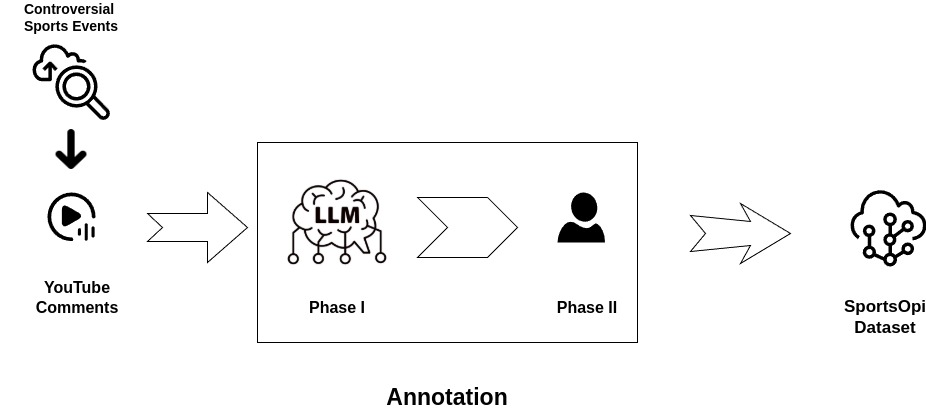
\includegraphics[width=0.5\textwidth]{SportsOpi.jpg} % Adjust width as needed
        \caption{Opinion Annotation  + Data Collection pipeline}
        \label{fig:labels}
    %\end{minipage}\hfill
%     \begin{minipage}{0.48\textwidth}
%         \centering
%         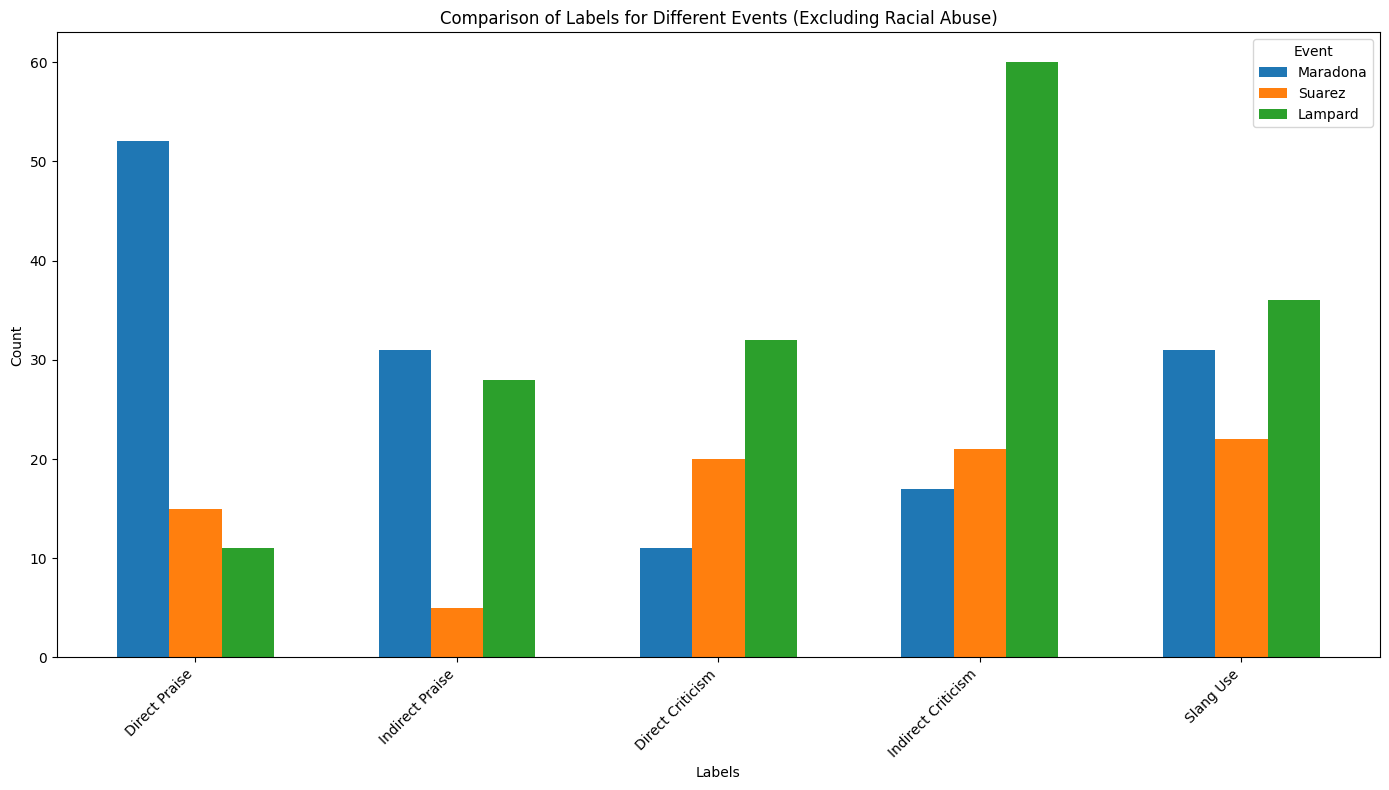
\includegraphics[width=\textwidth, keepaspectratio]{praise_and_criticism.jpg} % Adjust width as needed
%         \caption{Comparison of Types of Praise (Favor) and Criticism (Against) for a sample of 200 comments.}
%         \label{fig:praise_criticism}
%     \end{minipage}
 \end{figure}




\subsection{Opinion Annotation Pipeline}

\textbf{Figure 1} shows the process of our annotation pipeline for opinion mining.
The process for stance detection on our curated dataset consists of two stages as follows - 

\noindent {\bf Stage I:} After the \textbf{Data Collection Pipeline}, a dataset of comments from the chosen 6 sports controversies was created from which we sampled 200 random comments on which initial annotation was done using zero-shot prompt using Llama 3.1-8b Instruct model. 
LLMs were used as initial annotators \cite{tan2024largelanguagemodelsdata, pavlovic-poesio-2024-effectiveness} due to the popularity and success of the same in the synthetic data generation domain. 
Subsequently, we, to do the initial annotation ( \textit{Favor}, \textit{Against}, \textit{Neutral}, \textit{Irrelevant}).
It is important to keep in mind that the opinion labels were made with the subject of the controversy in mind, like Maradona from \textit{Maradona Hand of God} etc. We did the human verification with this idea in mind \footnote{\url{https://github.com/YuvrajSingh-mist/Public-Sports-Controversy/tree/master/data/PDFs}}. \\
{\bf Stage II:} Next, we humanely verified the labels as a result of {\bf Stage-I}. Thereafter, a sample of 20 comments were chosen, which became the basis of the few-shot prompt \footnote{\url{https://github.com/YuvrajSingh-mist/Public-Sports-Controversy/tree/master/data/Prompts}}. Only a few samples were used, since LLMs are prone to "overfit" to a specific type of data/samples provided in the k-shot prompt (if in excess).

This few-shot prompt was then used to annotate the entire dataset of comments with opinions. This was followed by thorough human verification.

\textbf{Table 1} shows the total number of comments, segregated into class-wise number of samples as well.
\textbf{Table 2 shows the result of our annotation process. It consists of sample of each of the four labels from our dataset.}

The following details the above-mentioned pipeline for each of the controversies used to constitute our dataset {\color{red}KRIPA: there should NOT be separate strategies for different events. If it is done, it needs to be justified}. - 

\begin{table}[h]
    \centering
    \small
    % \renewcommand{\arraystretch}{0.5} % Adjust row height
    % \setlength{\tabcolsep}{4pt}% Adjust column separation locally
    % \resizebox{\textwidth}{!}{ % Adjust table width to fit the page
    {
    \begin{tabular}{|c|c|c|c|c|c|} 
        \hline
        \textbf{Event} & \textbf{\#C} & \textbf{F} & \textbf{N} & \textbf{I} & \textbf{A} \\ 
        \hline
        Ashwin Mankading  & 3785  & 205 & 414 & 1734 & 1424 \\  
        Frank Lampard Ghost Goal & 13520 & 7000 & 1800 & 1100 & 3200 \\
        Johny Bairstow Runout & 6073 & 331 & 1936 & 1786 & 1987 \\
        Luis Suarez Handball & 11546 & 2400 & 2200 & 4200 & 2600 \\
        Maradona Hand of God & 5159 & 2100 & 900 & 1500 & 500 \\
        The Underarm Incident & 3676 & 330 & 126 & 1063 & 2113 \\
        \hline
        \textbf{Total} & \textbf{43759} & \textbf{12336} & \textbf{7376} & \textbf{11356} & \textbf{11824} \\
        \hline
    \end{tabular}
    }
    \caption{Name of comments, and class-wise distribution of comments.}
    \label{tab:merged_controversies}
\end{table}

\section{Results and Discussion}\label{sec:res_discuss}

Preliminary analysis indicates a significant division in public opinion across the six events within our dataset. 
Fine Tuning on our dataset improves the accuracy of the labels by a drastic margin along with other metrics such as F1 score, recall and precision as compared to the base instruct model.

\textbf{Table 3} shows the result of fine-tuning models on each of the six events.
Detailed results, including the distribution of stances (For, Against, Neutral, Irrelevant) and evaluation metrics (accuracy, precision, recall, F1-score).

% Wherever you want the table:
%\FloatBarrier % ensures all previous floats are processed
\begin{table*}[!htbp]
    \centering
    { % Start local grouping so formatting changes do not leak
      \small % Reduce font size
      \renewcommand{\arraystretch}{1.0}% Reduce row height
      \setlength{\tabcolsep}{3pt}% Reduce column separation
      \begin{tabular}{|c|p{3.5cm}|p{3.5cm}|p{3.5cm}|}
          \hline
          \textbf{Event} & \textbf{Favor} & \textbf{Against} & \textbf{Neutral} \\
          \hline
          {\textit{Frank}} 
           & Germans can't say anything about unsporting behavior.  
           & The 1966 ghost goal had to be paid for. 
           & This was more clear-cut than 1966. \\
          \hline
          {\textit{Suárez}} 
           & Morality loses, nice guys finish last.  
           & Hand of Satan. 
           & He will never step foot in Ghana. \\
          \hline
          {\textit{Maradona}} 
           & Goal 15 is something else...my favourite. 
           & Most cheating player in history. 
           & Can't pick between Maradona and Messi. \\
          \hline
          {\textit{Bairstow}} 
           & Not cheating, that's winning. 
           & Same old Aussies, always cheating. 
           & Lesson: ``pay attention''. \\
          \hline
          {\textit{Ashwin}} 
           & If bowler keeps foot inside, batsman can wait inside until ball is bowled. 
           & If you Mankad, you lack bowling skill. 
           & Ashwin expressed disappointment, never wanted that wicket. \\
          \hline
          {\textit{Underarm}} 
           & It was legal to bowl underarm then. 
           & Against rules! Couldn't they bowl normally? 
           & What were rules for underarm deliveries back then? \\
          \hline
      \end{tabular}
    } % End local grouping
    \caption{Examples of Favor, Against, and Neutral Comments for Controversial Events}
    \label{tab:event_comments}
\end{table*}
%\FloatBarrier % ensures the table is processed before subsequent content



% \vspace{5mm} % Add space before table

\begin{table*}[htbp]
    \centering
    \footnotesize % Use even smaller font size
    \setlength{\tabcolsep}{2pt} % Further reduce column separation
    \renewcommand{\arraystretch}{0.8} % Further reduce row height
    \begin{tabular}{|c|c|c|c|c|c|}
        \hline
        \textbf{Model} & \textbf{Event} & \textbf{Accuracy} & \textbf{Recall (micro)} & \textbf{Precision (micro)} & \textbf{F1 (micro)} \\
         \hline
         DeepSeek-8B (NFT) & \textit{Maradona} & 22.8\% & 23\% & 31\% & 9\% \\
         & \textit{Suarez} & 33.7\% & 34\% & 49\% & 24\% \\
         & \textit{Lampard} & 23\% & 23\% & 31\% & 9\% \\
          \hline
        DeepSeek-8B (FT) & \textit{Maradona} & 76.2\% & 76\% & 76\% & 76\% \\
         & \textit{Suarez} & 78\% & 78\% & 78\% & 78\% \\
         & \textit{Lampard} & 76.2\% & 76\% & 76\% & 76\% \\
        \hline
        Llama 3.1-8b (NFT) & \textit{Maradona} & 46.8\% & 46\% & 56\% & 40\% \\
         & \textit{Suarez} & 22.8\% & 23\% & 31\% & 9\% \\
         & \textit{Lampard} & 26.3\% & 26\% & 39\% & 25\% \\
         \hline
        Llama 3.1-8b (FT) & \textit{Maradona} & 79.0\% & 79\% & 78\% & 77\% \\
         & \textit{Suarez} & 79.5\% & 80\% & 79\% & 79\% \\
         & \textit{Lampard} & 71.6\% & 72\% & 72\% & 72\% \\
        \hline
    \end{tabular}
    \caption{Comparison of models with (FT)/without (NFT) fine-tuning on our dataset}
    \label{tab:student_info}
\end{table*}
\vspace{5mm}





\subsection{Detailed Analysis}


\begin{enumerate}
    \item \textit{Number of samples} (\textbf{Favor}, \textbf{Against}, \textbf{Neutral} and \textbf{Irrelevant})
    \begin{enumerate}
    \item The labels, \textit{Favor} and \textit{Against} is significantly higher for  \textit{Frank Lampard Ghost Goal} compared to other events with \textit{Favor} being comparatively higher, followed by \textit{Luiz Suarez Handball} event.
    \item The \textit number of samples for {Neutral} label is higher for \textit{Luis Suarez Handball} event.
    \item The label \textit{Irrelevant} is significantly higher for \textit{Luis Suarez Handball} event meaning the majority of the comments couldn't be classified into the other three labels.
   
    \end{enumerate}
    \item \textit{Variations of Praise and Criticism}
    \begin{enumerate}
        \item Instances of \textit{Direct Criticism} is highest for \textit{Maradona Hand of God} event.
        \item \textit{Direct Praise} accounts highest for \textit{Luis Suarez Handball} with equal instances for \textit{Maradona Hand of God} and \textit{Frank Lampard Ghost Goal}.
        \item For \textit{Indirect Criticism}, \textit{Frank Lampard Ghost Goal} is highest followed by \textit{Maradona Hand of God}.
        \item In terms of \textit{Favor} label (Direct + Indirect Praise), Frank Lampard event is highest, followed by Maradona and then by Luis Suarez events.
        \item  Similarly, for \textit{Against} label (Direct + Indirect Criticism), Maradona event's count is highest followed by Frank Lampard and then Luis Suarez events.
    
    \end{enumerate}
    
     Overall, \textit{Frank Lampard Ghost Goal} event is highly favoured as well as resented by the public. A balance between the three opinions can be found in \textit{Luis Suarez Handball} event.



\item \textit{Indepth analysis of stance labels}
        \begin{enumerate}
            \item We further investigated the primary stance labels, especially \textbf{Favor} and \textbf{Against}, by introducing more granular sub-categories: \textbf{Direct Praise}, \textbf{Indirect Praise}, \textbf{Direct Criticism}, and \textbf{Indirect Criticism}, along with tracking \textbf{Slang Use} and \textbf{Racial Abuse}. This allowed for a finer understanding of how different types of expressions correlate with overall sentiment across the datasets.

            % --- Summary Findings Start Here (as a nested list item) ---
            % \item Key relationships observed between these granular sub-categories and the main sentiment labels (referencing data from Tables 4, 5, and 6  include:
                % \begin{itemize} % Start list for each event/individual
                    \item \textbf{Maradona Hand of God Event (Ref: Table 4 \footnote{\url{https://github.com/YuvrajSingh-mist/Public-Sports-Controversy/blob/master/data/PDFs/Tables.pdf}})):}
                        % \begin{itemize}
                             \textit{Clear Alignment:} Direct Praise (I=1) aligns 100\% with \textbf{Favor} (E=0); Direct Criticism (H=1) aligns 100\% with \textbf{Against} (E=1).
                            \textit{Ambiguous Alignment:} Indirect Praise (K=1), Indirect Criticism (J=1), and Slang Use (L=1) are spread across multiple labels.
                          \textit{Rare Instance:} Racial Abuse (M=1) appeared infrequently under both \textbf{Favor} and \textbf{Against}.
                        % \end{itemize}

                    \item \textbf{Luis Suarez Handball Event (Ref: Table 5):}
                        % \begin{itemize}
                             \textit{Strong Alignment:} Direct Criticism (I=1) shows 94\% alignment with \textbf{Against} (D=1); Direct Praise (J=1) shows 78\% alignment with \textbf{Favor} (D=0); Racial Abuse (N=1) shows 71\% alignment with \textbf{Against} (D=1).
                           \textit{Weak Alignment:} Indirect Criticism (K=1) and Slang Use (M=1) lacked strong correlation with a single label.
                        % \end{itemize}

                    \item \textbf{Frank Lampard Ghost Goal Event (Ref: Table 6):}
                         % \begin{itemize}
                             \textit{Clear Alignment:} Direct Criticism (I) aligns 100\% with \textbf{Against} (H=1); Direct Praise (J) aligns 100\% with \textbf{Favor} (H=0).
                             \textit{Notable Trends:} Approx. 54\% of Indirect Criticism (K) comments were labeled \textbf{Favor} (H=0); Approx. 57\% of Slang Use (M) comments were labeled \textbf{Against} (H=1).
                        % \end{itemize}
                % \end{itemize} % End list for each event/individual
            % --- Summary Findings End Here ---

        \end{enumerate} % This is the \end{enumerate} before which the content was added
% (End of the outer \item \textit{Indepth analysis...})
      
 \item \textit{Probing Analysis of LLM outputs}

     

 
     We ran probing analysis \cite{orgad2024llms} on the attention outputs of the fine-tuned (denoted as positive class) and non-fine-tuned (negative class) versions of the Llama 3.1-8 b-Instruct model, denoted by Fig. 2 and 3, respectively (non-fine-tuned or the negative class \href{https://github.com/YuvrajSingh-mist/Public-Sports-Controversy/blob/master/data/PDFs/Tables.pdf}{here}).


     \begin{figure}[ht]
         \centering
         \begin{minipage}{0.35\textwidth}
             \centering
             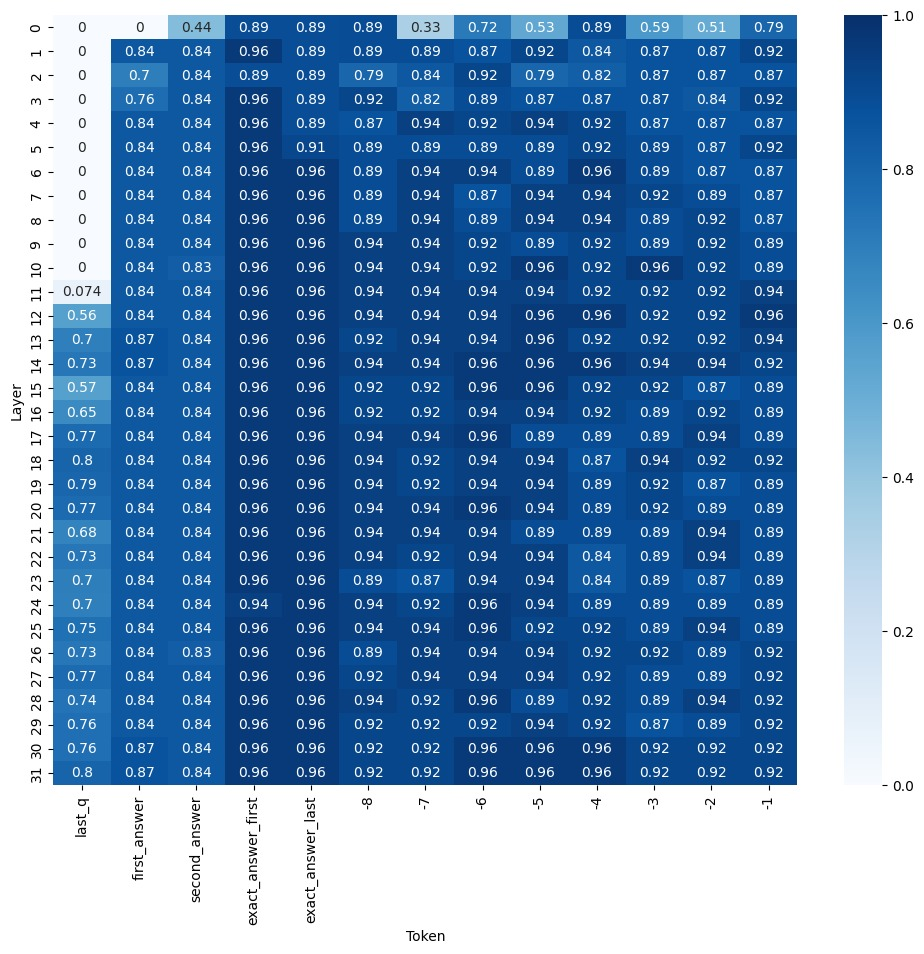
\includegraphics[width=\linewidth]{frank-positive-class.jpg}
             \caption{\footnotesize Frank Lampard Ghost Goal (Fine Tuned)}
             \label{fig:frank-positive-class}
         \end{minipage}
         \hfill
         \begin{minipage}{0.35\textwidth}
             \centering
             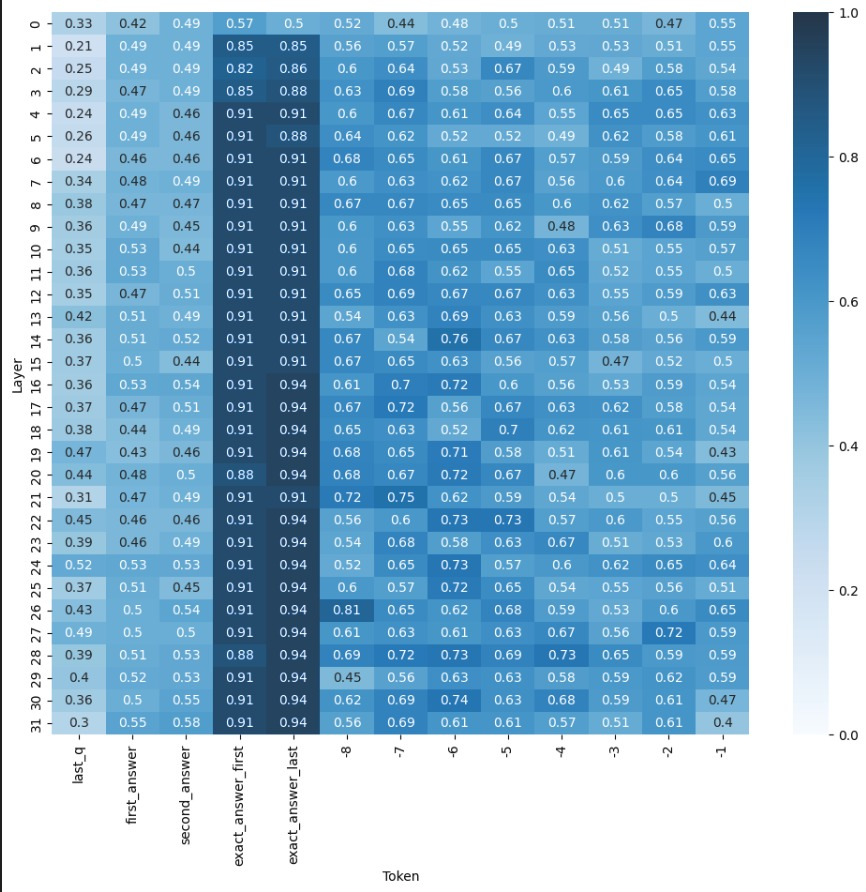
\includegraphics[width=\linewidth]{Suarez-positive-probing.jpg}
             \caption{\footnotesize Luis Suarez Handball (Fine Tuned)}
             \label{fig:suarez-positive-probing}
         \end{minipage}
         \caption{\footnotesize Attention heatmaps for fine-tuned LLama model.}
         \label{fig:positive-class-heatmaps}
     \end{figure}

     The attention outputs is particularly high for the tokens \texttt{exact\_answer\_first} and \texttt{exact\_answer\_last} for fine tuned model for majority of the layers, while for the non fine tuned one, it is high for all the tokens and layers, not consolidating to tokens particular to the answer to be generated.
     
     These heatmaps were generated by resp. F1 scores of a trained logistic classifier on attention outputs (fine tuned and non-fine-tuned model) only with accuracies 82\% and 23\% resp. for both the model.
     Due to high F1 and accuracy score for the fine-tuned models, we termed the labels generated by it to be a 'positive class' and for the other model to be a 'negative class' (low corresponding scores).
     
     We can see that the heatmap for the positive class or fine tuned models has high attention outputs for the tokens corresponding to the labels to be generated or the answer in particular, while it attends to every token for the non-fine-tuned or negative class model, not focusing on the labels or the answer generation tokens aforementioned particularly.
    
\end{enumerate}

\section{Conclusion}
This study highlights the role of social media in shaping public perception of sports controversies. Integrating automated data extraction and stance detection provides a comprehensive view of audience sentiment. Future enhancements will aim to improve accuracy and broaden the scope of analysis.



\if 0
\section{Template Overview}
As noted in the introduction, the ``\verb|acmart|'' document class can
be used to prepare many different kinds of documentation --- a
double-anonymous initial submission of a full-length technical paper, a
two-page SIGGRAPH Emerging Technologies abstract, a ``camera-ready''
journal article, a SIGCHI Extended Abstract, and more --- all by
selecting the appropriate {\itshape template style} and {\itshape
  template parameters}.

This document will explain the major features of the document
class. For further information, the {\itshape \LaTeX\ User's Guide} is
available from
\url{https://www.acm.org/publications/proceedings-template}.

\subsection{Template Styles}

The primary parameter given to the ``\verb|acmart|'' document class is
the {\itshape template style} which corresponds to the kind of publication
or SIG publishing the work. This parameter is enclosed in square
brackets and is a part of the {\verb|documentclass|} command:
\begin{verbatim}
  \documentclass[STYLE]{acmart}
\end{verbatim}

Journals use one of three template styles. All but three ACM journals
use the {\verb|acmsmall|} template style:
\begin{itemize}
\item {\texttt{acmsmall}}: The default journal template style.
\item {\texttt{acmlarge}}: Used by JOCCH and TAP.
\item {\texttt{acmtog}}: Used by TOG.
\end{itemize}

The majority of conference proceedings documentation will use the {\verb|acmconf|} template style.
\begin{itemize}
\item {\texttt{sigconf}}: The default proceedings template style.
\item{\texttt{sigchi}}: Used for SIGCHI conference articles.
\item{\texttt{sigplan}}: Used for SIGPLAN conference articles.
\end{itemize}

\subsection{Template Parameters}

In addition to specifying the {\itshape template style} to be used in
formatting your work, there are a number of {\itshape template parameters}
which modify some part of the applied template style. A complete list
of these parameters can be found in the {\itshape \LaTeX\ User's Guide.}

Frequently-used parameters, or combinations of parameters, include:
\begin{itemize}
\item {\texttt{anonymous,review}}: Suitable for a ``double-anonymous''
  conference submission. Anonymizes the work and includes line
  numbers. Use with the \texttt{\string\acmSubmissionID} command to print the
  submission's unique ID on each page of the work.
\item{\texttt{authorversion}}: Produces a version of the work suitable
  for posting by the author.
\item{\texttt{screen}}: Produces colored hyperlinks.
\end{itemize}

This document uses the following string as the first command in the
source file:
\begin{verbatim}
\documentclass[sigconf]{acmart}
\end{verbatim}

\section{Modifications}

Modifying the template --- including but not limited to: adjusting
margins, typeface sizes, line spacing, paragraph and list definitions,
and the use of the \verb|\vspace| command to manually adjust the
vertical spacing between elements of your work --- is not allowed.

{\bfseries Your document will be returned to you for revision if
  modifications are discovered.}

\section{Typefaces}

The ``\verb|acmart|'' document class requires the use of the
``Libertine'' typeface family. Your \TeX\ installation should include
this set of packages. Please do not substitute other typefaces. The
``\verb|lmodern|'' and ``\verb|ltimes|'' packages should not be used,
as they will override the built-in typeface families.

\section{Title Information}

The title of your work should use capital letters appropriately -
\url{https://capitalizemytitle.com/} has useful rules for
capitalization. Use the {\verb|title|} command to define the title of
your work. If your work has a subtitle, define it with the
{\verb|subtitle|} command.  Do not insert line breaks in your title.

If your title is lengthy, you must define a short version to be used
in the page headers, to prevent overlapping text. The \verb|title|
command has a ``short title'' parameter:
\begin{verbatim}
  \title[short title]{full title}
\end{verbatim}

\section{Authors and Affiliations}

Each author must be defined separately for accurate metadata
identification.  As an exception, multiple authors may share one
affiliation. Authors' names should not be abbreviated; use full first
names wherever possible. Include authors' e-mail addresses whenever
possible.

Grouping authors' names or e-mail addresses, or providing an ``e-mail
alias,'' as shown below, is not acceptable:
\begin{verbatim}
  \author{Brooke Aster, David Mehldau}
  \email{dave,judy,steve@university.edu}
  \email{firstname.lastname@phillips.org}
\end{verbatim}

The \verb|authornote| and \verb|authornotemark| commands allow a note
to apply to multiple authors --- for example, if the first two authors
of an article contributed equally to the work.

If your author list is lengthy, you must define a shortened version of
the list of authors to be used in the page headers, to prevent
overlapping text. The following command should be placed just after
the last \verb|\author{}| definition:
\begin{verbatim}
  \renewcommand{\shortauthors}{McCartney, et al.}
\end{verbatim}
Omitting this command will force the use of a concatenated list of all
of the authors' names, which may result in overlapping text in the
page headers.

The article template's documentation, available at
\url{https://www.acm.org/publications/proceedings-template}, has a
complete explanation of these commands and tips for their effective
use.

Note that authors' addresses are mandatory for journal articles.

\section{Rights Information}

Authors of any work published by ACM will need to complete a rights
form. Depending on the kind of work, and the rights management choice
made by the author, this may be copyright transfer, permission,
license, or an OA (open access) agreement.

Regardless of the rights management choice, the author will receive a
copy of the completed rights form once it has been submitted. This
form contains \LaTeX\ commands that must be copied into the source
document. When the document source is compiled, these commands and
their parameters add formatted text to several areas of the final
document:
\begin{itemize}
\item the ``ACM Reference Format'' text on the first page.
\item the ``rights management'' text on the first page.
\item the conference information in the page header(s).
\end{itemize}

Rights information is unique to the work; if you are preparing several
works for an event, make sure to use the correct set of commands with
each of the works.

The ACM Reference Format text is required for all articles over one
page in length, and is optional for one-page articles (abstracts).

\section{CCS Concepts and User-Defined Keywords}

Two elements of the ``acmart'' document class provide powerful
taxonomic tools for you to help readers find your work in an online
search.

The ACM Computing Classification System ---
\url{https://www.acm.org/publications/class-2012} --- is a set of
classifiers and concepts that describe the computing
discipline. Authors can select entries from this classification
system, via \url{https://dl.acm.org/ccs/ccs.cfm}, and generate the
commands to be included in the \LaTeX\ source.

User-defined keywords are a comma-separated list of words and phrases
of the authors' choosing, providing a more flexible way of describing
the research being presented.

CCS concepts and user-defined keywords are required for for all
articles over two pages in length, and are optional for one- and
two-page articles (or abstracts).

\section{Sectioning Commands}

Your work should use standard \LaTeX\ sectioning commands:
\verb|\section|, \verb|\subsection|, \verb|\subsubsection|,
\verb|\paragraph|, and \verb|\subparagraph|. The sectioning levels up to
\verb|\subsusection| should be numbered; do not remove the numbering
from the commands.

Simulating a sectioning command by setting the first word or words of
a paragraph in boldface or italicized text is {\bfseries not allowed.}

Below are examples of sectioning commands.

\subsection{Subsection}
\label{sec:subsection}

This is a subsection.

\subsubsection{Subsubsection}
\label{sec:subsubsection}

This is a subsubsection.

\paragraph{Paragraph}

This is a paragraph.

\subparagraph{Subparagraph}

This is a subparagraph.

\section{Tables}

The ``\verb|acmart|'' document class includes the ``\verb|booktabs|''
package --- \url{https://ctan.org/pkg/booktabs} --- for preparing
high-quality tables.

Table captions are placed {\itshape above} the table.

Because tables cannot be split across pages, the best placement for
them is typically the top of the page nearest their initial cite.  To
ensure this proper ``floating'' placement of tables, use the
environment \textbf{table} to enclose the table's contents and the
table caption.  The contents of the table itself must go in the
\textbf{tabular} environment, to be aligned properly in rows and
columns, with the desired horizontal and vertical rules.  Again,
detailed instructions on \textbf{tabular} material are found in the
\textit{\LaTeX\ User's Guide}.

Immediately following this sentence is the point at which
Table~\ref{tab:freq} is included in the input file; compare the
placement of the table here with the table in the printed output of
this document.

\begin{table}
  \caption{Frequency of Special Characters}
  \label{tab:freq}
  \begin{tabular}{ccl}
    \toprule
    Non-English or Math&Frequency&Comments\\
    \midrule
    \O & 1 in 1,000& For Swedish names\\
    $\pi$ & 1 in 5& Common in math\\
    \$ & 4 in 5 & Used in business\\
    $\Psi^2_1$ & 1 in 40,000& Unexplained usage\\
  \bottomrule
\end{tabular}
\end{table}

To set a wider table, which takes up the whole width of the page's
live area, use the environment \textbf{table} to enclose the table's
contents and the table caption.  As with a single-column table, this
wide table will ``float'' to a location deemed more
desirable. Immediately following this sentence is the point at which
Table~\ref{tab:commands} is included in the input file; again, it is
instructive to compare the placement of the table here with the table
in the printed output of this document.

\begin{table}
  \caption{Some Typical Commands}
  \label{tab:commands}
  \begin{tabular}{ccl}
    \toprule
    Command &A Number & Comments\\
    \midrule
    \texttt{{\char'134}author} & 100& Author \\
    \texttt{{\char'134}table}& 300 & For tables\\
    \texttt{{\char'134}table}& 400& For wider tables\\
    \bottomrule
  \end{tabular}
\end{table}

Always use midrule to separate table header rows from data rows, and
use it only for this purpose. This enables assistive technologies to
recognise table headers and support their users in navigating tables
more easily.

\section{Math Equations}
You may want to display math equations in three distinct styles:
inline, numbered or non-numbered display.  Each of the three are
discussed in the next sections.

\subsection{Inline (In-text) Equations}
A formula that appears in the running text is called an inline or
in-text formula.  It is produced by the \textbf{math} environment,
which can be invoked with the usual
\texttt{{\char'134}begin\,\ldots{\char'134}end} construction or with
the short form \texttt{\$\,\ldots\$}. You can use any of the symbols
and structures, from $\alpha$ to $\omega$, available in
\LaTeX~\cite{Lamport:LaTeX}; this section will simply show a few
examples of in-text equations in context. Notice how this equation:
\begin{math}
  \lim_{n\rightarrow \infty}x=0
\end{math},
set here in in-line math style, looks slightly different when
set in display style.  (See next section).

\subsection{Display Equations}
A numbered display equation---one set off by vertical space from the
text and centered horizontally---is produced by the \textbf{equation}
environment. An unnumbered display equation is produced by the
\textbf{displaymath} environment.

Again, in either environment, you can use any of the symbols and
structures available in \LaTeX\@; this section will just give a couple
of examples of display equations in context.  First, consider the
equation, shown as an inline equation above:
\begin{equation}
  \lim_{n\rightarrow \infty}x=0
\end{equation}
Notice how it is formatted somewhat differently in
the \textbf{displaymath}
environment.  Now, we'll enter an unnumbered equation:
\begin{displaymath}
  \sum_{i=0}^{\infty} x + 1
\end{displaymath}
and follow it with another numbered equation:
\begin{equation}
  \sum_{i=0}^{\infty}x_i=\int_{0}^{\pi+2} f
\end{equation}
just to demonstrate \LaTeX's able handling of numbering.

\section{Figures}

The ``\verb|figure|'' environment should be used for figures. One or
more images can be placed within a figure. If your figure contains
third-party material, you must clearly identify it as such, as shown
in the example below.
\begin{figure}[h]
  \centering
  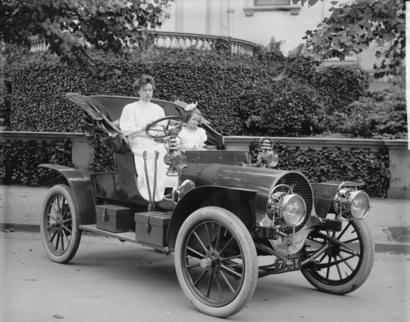
\includegraphics[width=\linewidth]{sample-franklin}
  \caption{1907 Franklin Model D roadster. Photograph by Harris \&
    Ewing, Inc. [Public domain], via Wikimedia
    Commons. (\url{https://goo.gl/VLCRBB}).}
  \Description{A woman and a girl in white dresses sit in an open car.}
\end{figure}

Your figures should contain a caption which describes the figure to
the reader.

Figure captions are placed {\itshape below} the figure.

Every figure should also have a figure description unless it is purely
decorative. These descriptions convey what’s in the image to someone
who cannot see it. They are also used by search engine crawlers for
indexing images, and when images cannot be loaded.

A figure description must be unformatted plain text less than 2000
characters long (including spaces).  {\bfseries Figure descriptions
  should not repeat the figure caption – their purpose is to capture
  important information that is not already provided in the caption or
  the main text of the paper.} For figures that convey important and
complex new information, a short text description may not be
adequate. More complex alternative descriptions can be placed in an
appendix and referenced in a short figure description. For example,
provide a data table capturing the information in a bar chart, or a
structured list representing a graph.  For additional information
regarding how best to write figure descriptions and why doing this is
so important, please see
\url{https://www.acm.org/publications/taps/describing-figures/}.

\subsection{The ``Teaser Figure''}

A ``teaser figure'' is an image, or set of images in one figure, that
are placed after all author and affiliation information, and before
the body of the article, spanning the page. If you wish to have such a
figure in your article, place the command immediately before the
\verb|\maketitle| command:
\begin{verbatim}
  \begin{teaserfigure}
    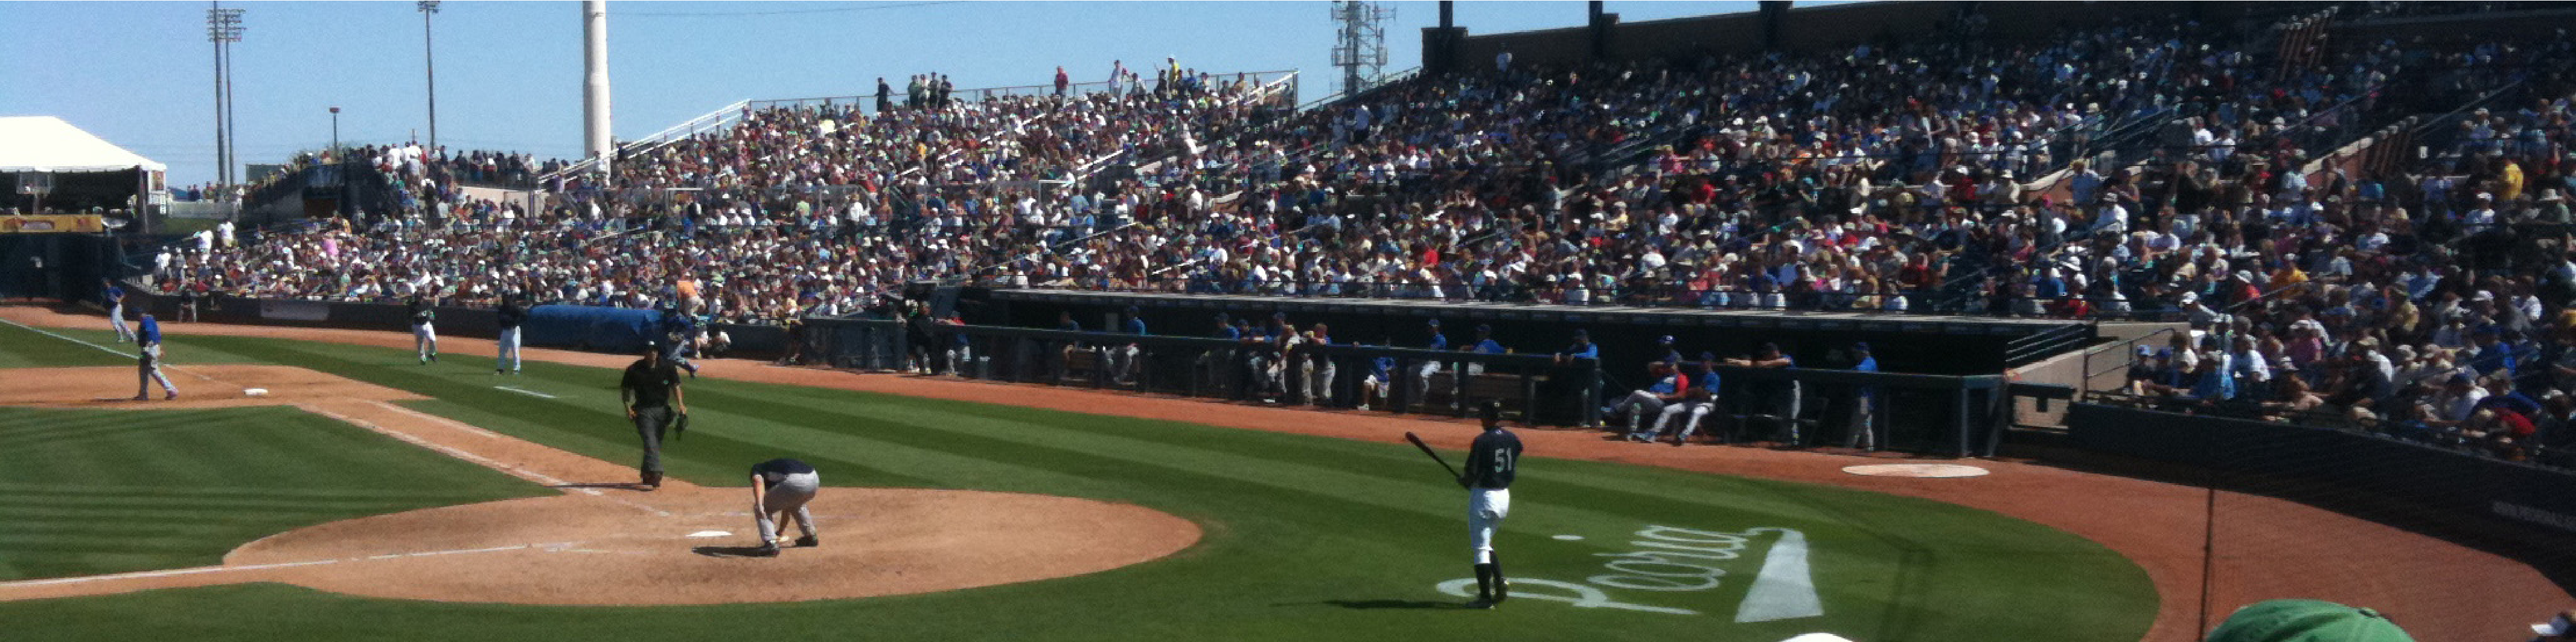
\includegraphics[width=\textwidth]{sampleteaser}
    \caption{figure caption}
    \Description{figure description}
  \end{teaserfigure}
\end{verbatim}

\section{Citations and Bibliographies}

The use of \BibTeX\ for the preparation and formatting of one's
references is strongly recommended. Authors' names should be complete
--- use full first names (``Donald E. Knuth'') not initials
(``D. E. Knuth'') --- and the salient identifying features of a
reference should be included: title, year, volume, number, pages,
article DOI, etc.

The bibliography is included in your source document with these two
commands, placed just before the \verb|\end{document}| command:
\begin{verbatim}
  \bibliographystyle{ACM-Reference-Format}
  \bibliography{bibfile}
\end{verbatim}
where ``\verb|bibfile|'' is the name, without the ``\verb|.bib|''
suffix, of the \BibTeX\ file.

Citations and references are numbered by default. A small number of
ACM publications have citations and references formatted in the
``author year'' style; for these exceptions, please include this
command in the {\bfseries preamble} (before the command
``\verb|\begin{document}|'') of your \LaTeX\ source:
\begin{verbatim}
  \citestyle{acmauthoryear}
\end{verbatim}


  Some examples.  A paginated journal article \cite{Abril07}, an
  enumerated journal article \cite{Cohen07}, a reference to an entire
  issue \cite{JCohen96}, a monograph (whole book) \cite{Kosiur01}, a
  monograph/whole book in a series (see 2a in spec. document)
  \cite{Harel79}, a divisible-book such as an anthology or compilation
  \cite{Editor00} followed by the same example, however we only output
  the series if the volume number is given \cite{Editor00a} (so
  Editor00a's series should NOT be present since it has no vol. no.),
  a chapter in a divisible book \cite{Spector90}, a chapter in a
  divisible book in a series \cite{Douglass98}, a multi-volume work as
  book \cite{Knuth97}, a couple of articles in a proceedings (of a
  conference, symposium, workshop for example) (paginated proceedings
  article) \cite{Andler79, Hagerup1993}, a proceedings article with
  all possible elements \cite{Smith10}, an example of an enumerated
  proceedings article \cite{VanGundy07}, an informally published work
  \cite{Harel78}, a couple of preprints \cite{Bornmann2019,
    AnzarootPBM14}, a doctoral dissertation \cite{Clarkson85}, a
  master's thesis: \cite{anisi03}, an online document / world wide web
  resource \cite{Thornburg01, Ablamowicz07, Poker06}, a video game
  (Case 1) \cite{Obama08} and (Case 2) \cite{Novak03} and \cite{Lee05}
  and (Case 3) a patent \cite{JoeScientist001}, work accepted for
  publication \cite{rous08}, 'YYYYb'-test for prolific author
  \cite{SaeediMEJ10} and \cite{SaeediJETC10}. Other cites might
  contain 'duplicate' DOI and URLs (some SIAM articles)
  \cite{Kirschmer:2010:AEI:1958016.1958018}. Boris / Barbara Beeton:
  multi-volume works as books \cite{MR781536} and \cite{MR781537}. A
  couple of citations with DOIs:
  \cite{2004:ITE:1009386.1010128,Kirschmer:2010:AEI:1958016.1958018}. Online
  citations: \cite{TUGInstmem, Thornburg01, CTANacmart}.
  Artifacts: \cite{R} and \cite{UMassCitations}.

\section{Acknowledgments}

Identification of funding sources and other support, and thanks to
individuals and groups that assisted in the research and the
preparation of the work should be included in an acknowledgment
section, which is placed just before the reference section in your
document.

This section has a special environment:
\begin{verbatim}
  \begin{acks}
  ...
  \end{acks}
\end{verbatim}
so that the information contained therein can be more easily collected
during the article metadata extraction phase, and to ensure
consistency in the spelling of the section heading.

Authors should not prepare this section as a numbered or unnumbered {\verb|\section|}; please use the ``{\verb|acks|}'' environment.

\section{Appendices}

If your work needs an appendix, add it before the
``\verb|\end{document}|'' command at the conclusion of your source
document.

Start the appendix with the ``\verb|appendix|'' command:
\begin{verbatim}
  \appendix
\end{verbatim}
and note that in the appendix, sections are lettered, not
numbered. This document has two appendices, demonstrating the section
and subsection identification method.

\section{Multi-language papers}

Papers may be written in languages other than English or include
titles, subtitles, keywords and abstracts in different languages (as a
rule, a paper in a language other than English should include an
English title and an English abstract).  Use \verb|language=...| for
every language used in the paper.  The last language indicated is the
main language of the paper.  For example, a French paper with
additional titles and abstracts in English and German may start with
the following command
\begin{verbatim}
\documentclass[sigconf, language=english, language=german,
               language=french]{acmart}
\end{verbatim}

The title, subtitle, keywords and abstract will be typeset in the main
language of the paper.  The commands \verb|\translatedXXX|, \verb|XXX|
begin title, subtitle and keywords, can be used to set these elements
in the other languages.  The environment \verb|translatedabstract| is
used to set the translation of the abstract.  These commands and
environment have a mandatory first argument: the language of the
second argument.  See \verb|sample-sigconf-i13n.tex| file for examples
of their usage.

\section{SIGCHI Extended Abstracts}

The ``\verb|sigchi-a|'' template style (available only in \LaTeX\ and
not in Word) produces a landscape-orientation formatted article, with
a wide left margin. Three environments are available for use with the
``\verb|sigchi-a|'' template style, and produce formatted output in
the margin:
\begin{description}
\item[\texttt{sidebar}:]  Place formatted text in the margin.
\item[\texttt{marginfigure}:] Place a figure in the margin.
\item[\texttt{margintable}:] Place a table in the margin.
\end{description}

%%
%% The acknowledgments section is defined using the "acks" environment
%% (and NOT an unnumbered section). This ensures the proper
%% identification of the section in the article metadata, and the
%% consistent spelling of the heading.
\begin{acks}
To Robert, for the bagels and explaining CMYK and color spaces.
\end{acks}
\fi
%%
%% The next two lines define the bibliography style to be used, and
%% the bibliography file.
\bibliographystyle{ACM-Reference-Format}
\bibliography{sample-base}


%%
%% If your work has an appendix, this is the place to put it.

\if 0
\appendix

\section{Research Methods}

\subsection{Part One}

Lorem ipsum dolor sit amet, consectetur adipiscing elit. Morbi
malesuada, quam in pulvinar varius, metus nunc fermentum urna, id
sollicitudin purus odio sit amet enim. Aliquam ullamcorper eu ipsum
vel mollis. Curabitur quis dictum nisl. Phasellus vel semper risus, et
lacinia dolor. Integer ultricies commodo sem nec semper.

\subsection{Part Two}

Etiam commodo feugiat nisl pulvinar pellentesque. Etiam auctor sodales
ligula, non varius nibh pulvinar semper. Suspendisse nec lectus non
ipsum convallis congue hendrerit vitae sapien. Donec at laoreet
eros. Vivamus non purus placerat, scelerisque diam eu, cursus
ante. Etiam aliquam tortor auctor efficitur mattis.

\section{Online Resources}

Nam id fermentum dui. Suspendisse sagittis tortor a nulla mollis, in
pulvinar ex pretium. Sed interdum orci quis metus euismod, et sagittis
enim maximus. Vestibulum gravida massa ut felis suscipit
congue. Quisque mattis elit a risus ultrices commodo venenatis eget
dui. Etiam sagittis eleifend elementum.

Nam interdum magna at lectus dignissim, ac dignissim lorem
rhoncus. Maecenas eu arcu ac neque placerat aliquam. Nunc pulvinar
massa et mattis lacinia.
\fi
\end{document}
\endinput